
\BiChapter{MA Thesis使用指南}{Use Guide of Ph.D Dissertation}
安装配置环境与编辑器选择:使用此模板需先下载TeX Live用以配置编译环境,还需下载TeXstudio作为编辑器。当TeX Live和TeXstudio下载好后可不用管TeX Live,直接在TeXstudio中编辑运行即可。\par
打开TeXstudio,点击菜单栏里的选项按钮,选择编辑TeXstudio,在构建里将默认编辑器设置成XeLaTex,再点击菜单栏里的文件选择打开选项打开DUT文件夹里的MA Thesis.tex文件,之后点击绿色的运行按钮进行首次编译运行,最后添加自己的内容进行论文撰写。
\BiSection{此Latex论文模板使用须知}{Basic Instructions for Using Latex}
(1)知道\textbackslash chapter\{\}是章开始的意思,在{}里面填入章节名称,然后在后面写上内容即可;同理\textbackslash section\{\}和\textbackslash subsection\{\}分别对应节、次节,用法同“章”;\par
(2)知道另起一段在一段内容结束后用\textbackslash par即可达到另起一段的目的;至于换行不用管会自动换行的;\par
(3)知道在什么地方填内容,参考模板中abstract、denotation、chapter1-6、app1、app2、pub、thanks、resume去填入自己论文的内容。\par
(4)论文中的封面、原创性申明和授权书、奇偶页页眉内容填写在DUT-thesis-grd.cls文件里进行编辑,需要论文作者找到对应位置进行内容更改,具体编辑位置如下图中红框部分所示:\par
论文封面内容编辑:\par
\begin{figure}[!ht]
	\centering
	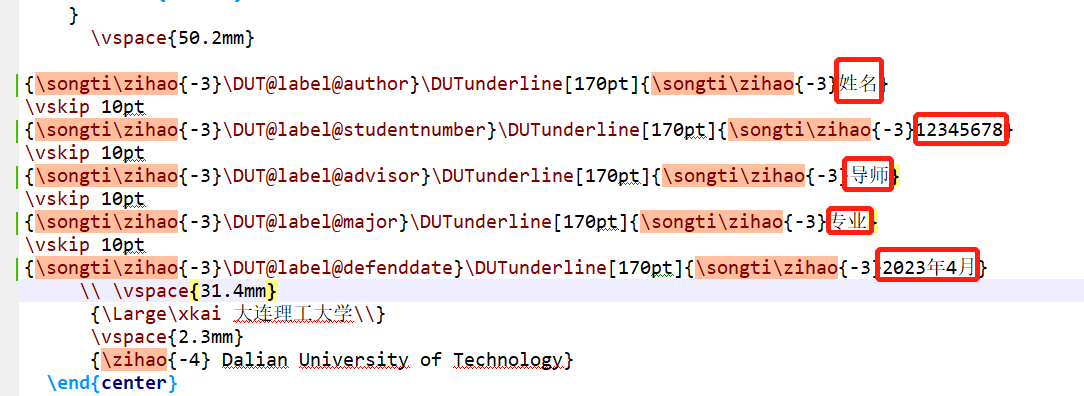
\includegraphics[width=0.9\textwidth]{figures/figure10}
	\bicaption{封面}{cover}  
\end{figure}
原创性申明和授权书内容编辑:\par
\begin{figure}[H]
	\centering
	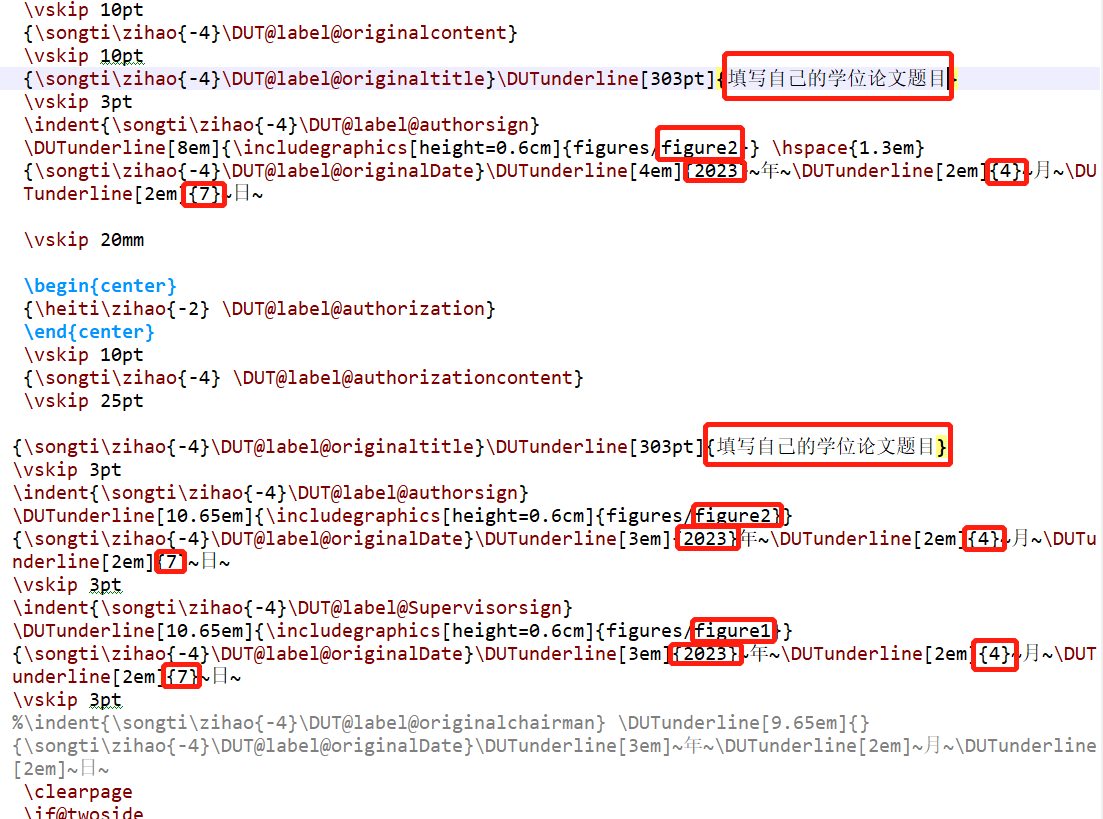
\includegraphics[width=0.8\textwidth,height=0.5\textwidth]{figures/figure11}
	\bicaption{申明}{statements}  
\end{figure}
奇偶页页眉编辑:\par
\begin{figure}[!ht]
	\centering
	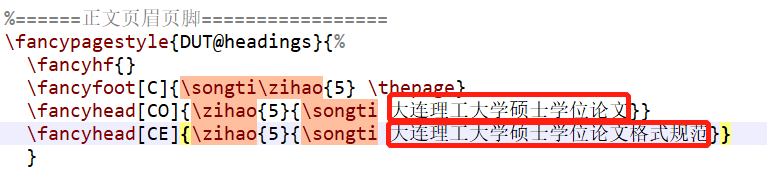
\includegraphics{figures/figure12}
	\bicaption{页眉}{header}  
\end{figure}
(5)要想用好latex进行论文写作,仅通过本文的介绍还不够,建议的学习资料如下:\url{https://github.com/BIT-thesis/LaTeX-materials}\par

